\documentclass[a4paper,11pt]{article}
\usepackage[english]{babel}
\usepackage[utf8]{inputenc}
\usepackage[T1]{fontenc}
\usepackage{graphicx}
\usepackage{amsmath}
\usepackage{tikz}
\usepackage{amsthm}
\usepackage{amssymb}
\usepackage{nicefrac}
\usepackage{tabularx}
\usepackage{cprotect}
\usepackage{wrapfig}
\usepackage{framed}
\usepackage{fancyvrb}
\usepackage{bm}
\usepackage{listings}
\usepackage{longtable}
\usepackage[left=25mm,right=25mm,bottom=25mm,top=25mm]{geometry} %left, right, bottom ,top, includeheadfoot
\usepackage{caption}
\usepackage{multicol}
\usepackage{subcaption}
\usepackage{nameref}
\usepackage{placeins} %Put command \floatbarrier in front of textpassage or other items, in front of which the desired content (i.e. images) shall be placed.
\usepackage[inline]{enumitem}
% \usepackage[parfill]{parskip}
%\usepackage{fancyhdr}
\usepackage{enumitem}
\usepackage{siunitx}
\newcounter{question}
\setcounter{question}{0}
\usepackage{blindtext}
\usepackage{hyperref} %To make document linked within.
\usepackage{cleveref}
\numberwithin{equation}{section}
\captionsetup{font=footnotesize,labelfont=bf}

\renewcommand{\theenumi}{(\arabic{enumi})}
\renewcommand\labelenumi{\theenumi} % Change enumerate style from 1. to (1) etc.
\renewcommand{\theenumiii}{(\arabic{enumiii})}
\renewcommand\labelenumiii{\theenumiii} % Change enumerate style from 1. to (1) etc.
\setlist{itemsep = 0.2pt}


\newcommand\matr[1]{\ensuremath{\boldsymbol{\mathbf{#1}}}}
\newcommand\vect[1]{\ensuremath{\bm{#1}}}
\newcommand\dint{\ensuremath{\int\displaylimits}}

%\DeclareSIUnit \parsec {pc}
%\DeclareSIUnit \magnitudes {mag}
\DeclareSIUnit \curie {Ci}

\title{Machine Learning\\ \vspace{0.2cm}\normalsize Questions and Answers}
\author{Daniel Zahnd}
\date{September 16, 2024 - \today}


\newtheorem{ass}{Assertion}

\begin{document}


\newcommand\Que[1]{%
   \leavevmode\par
   \stepcounter{question}
   \noindent
   \thequestion. \textbf{Q} --- #1\par}

\newcommand\Ans[2][]{%
    \leavevmode\par\noindent
   {\leftskip0pt
    \textbf{A} --- \textbf{#1}#2\par}}

\maketitle
%\thispagestyle{empty}
\tableofcontents
%\newpage

\pagenumbering{arabic}
\setcounter{page}{1}

\section{Preliminaries}
Usually, one deals with datasets containing of data $x \in \mathbb{R}^n$ associated to other data $y$ with $n \in \mathbb{N}$. The data $x$ can be scalar of vectorial, whereas the data $y$ can also be a scalar or vector. The data $x$ is either $y \in \mathbb{R}^q$ with $q \in \mathbb{R}$ or a number of a class $\{1,\dots,K\}$ for $K \in \mathbb{N}$. In the case where e.g. $y \in \mathbb{R}$, one speaks of a regression problem, whereas in the case where $y \in\{1,\dots,K\}$ are classes, one speaks of a classification task.

Usually, one has a dataset containing of various pairs of $x$ and $y$; to distinguish an instance of data from components of a vector, one writes $(x^{(i)}, y^{(i)})$ for an instance of a dataset containing of $m \in \mathbb{N}$ instances of data. For components of an instance of data $x^{(i)} \in \mathbb{R}^n$, one writes \begin{equation}
	x^{(i)} = \begin{pmatrix}
		x^{(i)}_1 \\ \vdots \\ x^{(i)}_n
	\end{pmatrix} \in \mathbb{R}^n.
\end{equation} For a whole dataset, one can write \begin{equation}
\{(x^{(i)}, y^{(i)})\}_{i=1,\dots,m} = \{(x^{(1)}, y^{(1)}), \dots , (x^{(m)}, y^{(m)})\}.
\end{equation}

The goal in machine learning is thus to find a function $h$ with associated tunable parameters $\theta$, that predicts $y$ based on $x$; hence one can write \begin{equation}
	h_\theta(x) = y.
\end{equation} The ultimate goal usually is to determine the parameters (weights) $\theta$; whereas for the shape or nature of the function $h$, one can usually make assumptions. The $h$ is reminiscent of ``hypothesis'' and thus of ``hypothesis'' function.

\subsection{Probability measures}
\subsubsection{Random variable}
A random variable is some quantity $x$, which can take a random value. Those random values follow a certain probability distribution, which is determined by the underlying process constituting the random variable.If the probability distribution of a random variable is known, the probability density $p(x)$ can be written down for the continuous and discrete cases as \begin{equation}
	\int_{-\infty}^{\infty}p(x)\,\mathrm{d}x = 1 \qquad \text{and} \qquad \sum_{i} p(x_i) = 1.
\end{equation}

\subsubsection{Expectation value}
The expectation value $\mathbb{E}(x) \doteq \bar{x}$ of a random variable $x$ for both the continuous and discrete case is defined as \begin{equation}
	\mathbb{E}(x) = \int_{-\infty}^{\infty}xp(x)\,\mathrm{d}x \qquad \text{and} \qquad \mathbb{E}(x) = \sum_{i}x_ip(x_i).
\end{equation}

\subsubsection{Variance, standard deviation and covariance}
The variance $\mathbb{V}(x)$ of a continuous or discrete random variable $x$ can be calculated by means of \begin{equation}
	\mathbb{V}(x) = \int_{-\infty}^{\infty} (x-\bar{x})^2p(x)\,\mathrm{d}x \qquad \text{and} \qquad \mathbb{V}(x) = \sum_{i} (x_i-\bar{x})^2p(x_i).
\end{equation}
The standard deviation $\sigma_x$ is defined as the square root of the variance, hence \begin{equation}
	\sigma_x = \sqrt{\mathbb{V}(x)}.
\end{equation}
Let now $x_1,\dots,x_n$ be random variables with associated probability densities $p(x_j)$, $j\in \{1,\dots,n\}$ and joint probability densities $p(x_i,x_j)$. Let furthermore be $\bar{x}_i = \mathbb{E}(x_i)$. The covariance $\mathbb{K}(x_i,x_j)$ of two random variables for the continuous and discrete case is defined as \begin{equation}\label{eq:covariance}
	\mathbb{K}(x_i,x_j) = \int_{-\infty}^{\infty}\int_{-\infty}^{\infty}(x_i-\bar{x}_i)(x_j-\bar{x}_j)p(x_i,x_j)\,\mathrm{d}x_i\,\mathrm{d}x_j
\end{equation} and \begin{equation}
	\mathbb{K}(x_i,x_j) = \sum_{k,l}(x_{i_k}-\bar{x}_i)(x_{j_l}-\bar{x}_j)p(x_{i_k},x_{j_l}).
\end{equation} In the context of covariance, one usually also defines the correlation coefficient $\rho(x_i,x_j)$ between two random variables as \begin{equation}\label{eq:correlationcoefficient}
	\rho(x_i,x_j) = \frac{\mathbb{K}(x_i,x_j)}{\sqrt{\mathbb{V}(x_i)\mathbb{V}(x_j)}} = \frac{\mathbb{K}(x_i,x_j)}{\sigma_{x_i}\sigma_{x_j}}.
\end{equation} % Definitions of expectation values and so on, and of Gaussian, Binomial, Poisson and Bernoulli distributions and why and when they are used

\subsection{Preliminary questions}
\Que{How is the uniform distribution defined?}
\Ans{
	Consider a continuous random variable $x$. The uniform probability distribution is defined by the probability density $p(x)$ as \begin{equation}
		p(x) = \mathcal{U}(x; a,b) = \begin{cases}
			\frac{1}{b-a} &, a \leq x \leq b \\
			0 &, \text{otherwise}
		\end{cases}
	\end{equation} where $a$ and $b$ define the domain of the distribution. The expectation value and the variance of the uniform distribution are given by \begin{equation}
		\mathbb{E}(x) = \frac{a+b}{2}, \quad \mathbb{V}(x) = \frac{1}{12}(b-a)^2.
	\end{equation} 
	
	The uniform distribution is used for processes with no prior knowledge about the probabilities of events. It is furthermore used to model processes, where all outcomes are equally likely to happen.
}

\Que{How is the standard normal distribution defined?}
\Ans{
	Consider a continuous random variable $x$. The standard normal probability distribution (Gaussian) is defined by the probability density $p(x)$ as \begin{equation}
		p(x) = \mathcal{N}(x;\mu,\sigma) = \frac{1}{\sqrt{2\pi}\sigma}e^{-\frac{(x-\mu)^2}{2\sigma^2}}
	\end{equation} where $\mu$ defines the expectation value and $\sigma$ the variance the distribution. The expectation value and the variance of the uniform distribution are given by \begin{equation}
		\mathbb{E}(x) = \mu, \quad \mathbb{V}(x) = \sigma^2.
	\end{equation} 
	
	The normal distribution is used for processes, which are influenced by an additive effect of a large number of different and independent influences modelled by arbitrary probability distributions. It pertains - with the uniform distribution - to the two default probability distributions to use, where little prior information about the modelled processes is available.
}

\Que{How is the Bernoulli distribution defined?}
\Ans{
	Consider a discrete random variable $x$. The Bernoulli probability distribution is defined by the probability density $p(x)$ as
	\begin{equation}
		p(x) = \mathcal{B}(x; p) =
		\begin{cases}
			p &, x = 1 \\
			1 - p &, x = 0 
		\end{cases},
	\end{equation}
	where $0 \leq p \leq 1$ is the probability of success (i.e., $x = 1$). The random variable $x$ takes on only two possible values: 1 (success) or 0 (failure).
	
	The expectation value and variance of the Bernoulli distribution are given by
	\begin{equation}
		\mathbb{E}(x) = p, \quad \mathbb{V}(x) = p(1 - p).
	\end{equation}
	
	The Bernoulli distribution models a single trial of an experiment where there are exactly two possible outcomes: success with probability $p$ and failure with probability $1 - p$. It is a fundamental building block of the binomial distribution, which models a sequence of independent Bernoulli trials.
}

\Que{How is the binomial distribution defined?}
\Ans{
	Consider a discrete random variable $x$. The binomial probability distribution is defined by the probability density $p(x)$ as \begin{equation}
		p(x) = \mathcal{B}(x;n,p) = \begin{cases}
			\binom{n}{x}p^x(1-p)^{n-x} &, x \in \{1,\dots,n\} \\
			0 &, \text{otherwise}
		\end{cases},
	\end{equation} where $n$ denotes the number of trials of an experiment and $p$ is the respective probability of success or failure of the outcome. The expectation value and the variance of the binomial distribution are given by \begin{equation}
		\mathbb{E}(x) = np, \quad \mathbb{V}(x) = np(1-p).
	\end{equation} 
	
	The binomial distribution is used to model processes that model a series of identical and independent experiments with exactly two possible outcomes, success or failure.
}

\Que{How is the Poisson distribution defined?}
\Ans{
	Consider a discrete random variable $x$. The Poisson probability distribution is defined by the probability density $p(x)$ as \begin{equation}
		p(x) = \mathcal{P}(x;\lambda) = \begin{cases}
			\frac{\lambda^x}{x!}e^{-\lambda} &, x \in \mathbb{N}_0 \\
			0 &, \text{otherwise}
		\end{cases},
	\end{equation} where $\lambda > 0$ defines both the expectation value and the variance. The expectation value and the variance of the Poisson distribution are given by \begin{equation}
		\mathbb{E}(x) = \lambda, \quad \mathbb{V}(x) = \lambda.
	\end{equation} 
	
	The Poisson distribution is - similarly to the binomial distribution - used to model processes that model a series of identical and independent experiments with exactly two possible outcomes, success or failure, but where the probability $p$ of success behaves as $p \rightarrow 0$ and where the number of trials $n$ behaves as $n\rightarrow \infty$.
}

\Que{How is the Poisson distribution defined?}
\Ans{
	Consider a discrete random variable $x$. The Poisson probability distribution is defined by the probability density $p(x)$ as \begin{equation}
		p(x) = \mathcal{P}(x;\lambda) = \begin{cases}
			\frac{\lambda^x}{x!}e^{-\lambda} &, x \in \mathbb{N}_0 \\
			0 &, \text{otherwise}
		\end{cases},
	\end{equation} where $\lambda > 0$ defines both the expectation value and the variance. The expectation value and the variance of the Poisson distribution are given by \begin{equation}
		\mathbb{E}(x) = \lambda, \quad \mathbb{V}(x) = \lambda.
	\end{equation} 
	
	The Poisson distribution is - similarly to the binomial distribution - used to model processes that model a series of identical and independent experiments with exactly two possible outcomes, success or failure, but where the probability $p$ of success behaves as $p \rightarrow 0$ and where the number of trials $n$ behaves as $n\rightarrow \infty$.
}

\Que{What is the popular definition of machine learning authored by Arthur Samuel in 1959?}
\Ans{According to Samuel, machine learning is the field of study that gives computers the ability to learn without being explicitly programmed. Explicitly programmed here means, that everything would be hard-coded, instead of rule-based programming.}

\Que{What is another popular definition of machine learning authored by Tom Michel in 1999?}
\Ans{
According to Michel, a well-posed machine learning problem may be described as follows: A computer program is said to learn from experience $E$ with respect to some tasks $T$ and performance measure $P$, if its performance at tasks $T$ as measured by performance $P$ improves with experience $E$.
}

\Que{Broadly speaking, which three types of machine learning algorithms are there?}
\Ans{Broadly speaking, there are three different categories of machine learning algorithms:
\begin{enumerate}
	\item Supervised learning: A machine learns how to make predictions about a specific target of interest, given some observations.
	\item Unsupervised learning: A machine learns how to find useful structures and patterns in given data by itself.
	\item Reinforcement learning: A machine has the ability to act and thus influence its own observations, thereby learning to make predictions to achieve a given goal.
\end{enumerate}

An example of supervised learning would be a classification task; that is to say to assign data to two or more given classes of objects depending on one or more variables. One could for example do this by means of linear or polynomial regression.

In comparison to supervised learning, unsupervised learning would for example try to separate data into two or more classes of objects, depending on what makes sense to the algorithm.

Reinforcement learning finally is about problems, where a sequence of decisions over time is required, where the basic idea is to implement a reward function as supervision to give the model a way to improve itself.
}

\Que{How does gradient descent work; and what is the difference between stochastic gradient descent and just gradient descent?}
\Ans{
	Gradient descent is one of the most useful and foundational techniques in machine learning; basically, it is about minimizing a loss function $J(\theta)$ with respect to weights (parameters) $\theta$ which belong to the chosen model.
	
	Hence, let now $J(\theta)$ be the loss function of a model, where $\theta = (\theta_1, \dots, \theta_n)^\top$ are the parameters of the model, which need to be optimized. The loss function might take a form as given in \cref{fig:gradientdescent}.
	\begin{figure}[h]
		\centering
		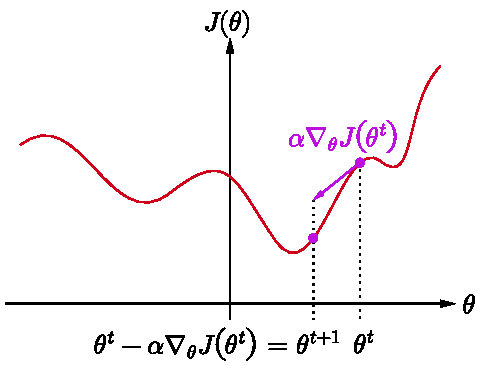
\includegraphics[width=0.4\textwidth]{figures/gradientdescent.pdf}
		\caption{Visualization of the gradient descent routine. Note, that $\theta$ is generally a vector; thus, the figure does only represent the general case in the case where $\theta$ is a scalar. If $\theta$ would consist of two components, the figure would be still visualizable in two dimensions on paper, but for higher dimensions in $\theta$, gradient descent may not be visualizable anymore on paper.}
		\label{fig:gradientdescent}
	\end{figure}
	Now, $\theta^t$ denotes the weights at iteration step $t \in \{1,\dots,T\}$ for a total iteration time $T$. Well, gradient descent updates the weights as \begin{equation}
		\theta^{t+1} = \theta^t - \alpha\nabla_\theta J(\theta^t),
	\end{equation} where the gradient is taken with respect to the weights $\theta$ and is evaluated at $\theta^t$, i.e. \begin{equation}
		\nabla_\theta = \sum_{j=1}^n e_j\partial_{\theta_j}.  \end{equation} In the case, where no confusion arises to which respect a gradient is taken, the subscript can also be left away. The parameter $\alpha$ is called the learning rate in machine learning and it has to be chosen such, that the algorithm does find the global, instead of just a local minimum of $J(\theta)$.
}

\Que{What is the rationale for the learning rate $\alpha$ in gradient descent?}
\Ans{
Consider \cref{fig:gradientdescentrationale}; it shows a curve $J(\theta)$ and a quadratic function $g(\theta) = \|\theta- \theta^t\|$. Now, one can Taylor expand the function $J(\theta)$ around
\begin{figure}[h]
	\centering
	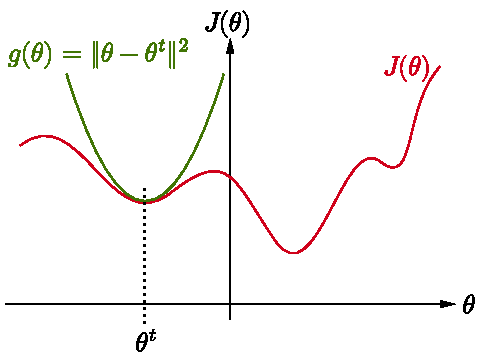
\includegraphics[width=0.4\textwidth]{figures/gradientdescentrationale.pdf}
	\caption{Rationale behind the gradient descent routine and the learning rate $\alpha$.}
	\label{fig:gradientdescentrationale}
\end{figure} % Lecture 3 about 55min in
an iteration step $\theta^t$ quite easily to first order in $\theta$ as \begin{equation}
	J(\theta) \approx J(\theta^t) + \nabla_\theta J(\theta^t)^\top (\theta - \theta^t).
\end{equation} Now, the second order term would involve the Hessian, which can be quite complicated. However, one can always add a quadratic term of the form $g(\theta)$, which is scaled by some parameter $\varepsilon$, such that the resulting approximation of $J(\theta)$ always stays above the exact function; the added term with $\varepsilon$ thus approximates the Hessian. One hence has \begin{equation}
J(\theta) \approx J(\theta^t) + \nabla_\theta J(\theta^t)^\top (\theta - \theta^t) + \frac{1}{2\varepsilon}\|\theta - \theta^t\|^2.
\end{equation} In order to find a minimum of this expression, one has to compute the gradient of the expression with respect to $\theta$, set it to zero and solve for $\theta$. From this, \begin{equation}
\nabla_\theta J(\theta) \approx 0 + \nabla_\theta J(\theta^t) + \frac{1}{\varepsilon}(\theta- \theta^t) \overset{!}{=} 0 \quad \Leftrightarrow \quad \theta = \theta^t - \varepsilon\nabla_\theta J(\theta^t)
\end{equation} follows. This is nothing but gradient descent, where $\varepsilon = \alpha$ is the learning rate. As one can see, the width $(2\varepsilon)^{-1}$ of the added quadratic term to the first order Taylor expansion of $J(\theta)$ is the inverse of the learning rate. If the learning rate is large, the width of the added quadratic term is very narrow.
}

\section{Supervised learning}
\subsection{Linear regression}
\subsubsection{Least mean squares} % Lecture 1
\Que{How can a most simple machine learning model performing affine regression be implemented?}
\Ans{
Let $x \in \mathbb{R}^n$ be a feature vector and $y \in \mathbb{R}$. Let furthermore $(x^{(i)}, y^{(i)})$ with $i \in \{1,\dots,m\}$ be a training dataset. Now, for affine regression, we can suggest a hypothesis function \begin{equation}
	h_{\theta}(x) = \theta_0 + \theta_1x_1 + \theta_2 x_2 + \dots + \theta_n x_n,
\end{equation} which, defining $x \doteq (1, x_1, x_2, \dots, x_n)^\top$, can be written more compactly as \begin{equation}
h_\theta(x) = \theta^\top x.
\end{equation} As a loss function to  minimize, it makes sense to take the Euclidean norm as a metric to measure ``closeness'' of the prediction $h_\theta(x^{(i)})$ to the actual value $y^{(i)}$, thus \begin{equation}
J(\theta) \doteq \frac{1}{2}\sum_{i=1}^{m}\|h_\theta(x^{(i)})-y^{(i)})\|^2= \frac{1}{2}\sum_{i=1}^{m}\|\theta^\top x^{(i)}-y^{(i)})\|^2.
\end{equation} The update rule for this regression task would be thus given by \begin{equation}
\theta^{t+1} = \theta^t - \alpha \nabla_\theta J(\theta) = \theta^t - \alpha \sum_{i=1}^{m}\left(\theta^\top x^{(i)}-y^{(i)}\right)x^{(i)}, 
\end{equation} where $\alpha \in \mathbb{R}$ is a suitably chosen learning rate. The proposed algorithm is called a least mean squares algorithm. This algorithm is equivalent to stating the optimal model parameters $\hat{\theta}$ as \begin{equation}
\hat{\theta} = \arg\min_\theta \left(\sum_{i=1}^m\left[\theta^\top x^{(i)}-y^{(i)}\right]^2\right).
\end{equation}
}

\Que{How can the least mean squares method be given in matrix form in the general case?}
\Ans{
Let $x \in \mathbb{R}^n$ be a feature vector and $y \in \mathbb{R}$. Let furthermore $(x^{(i)}, y^{(i)})$ with $i \in \{1,\dots,m\}$ be a training dataset. Define a matrix $X$, such that $(x^{(i)})^\top$ is the $i$-th row and a matrix $Y$, such that $y^{(i)}$ is also the $i$-th row, namely \begin{equation}
	X \doteq \begin{pmatrix}
		1 & (x^{(1)})^\top \\
		\vdots & \vdots \\
		1 & (x^{(m)})^\top
	\end{pmatrix}, \qquad Y \doteq \begin{pmatrix}
	y^{(1)} \\
	\vdots \\
	y^{(m)}
	\end{pmatrix}.
\end{equation} Hereby, a column of ones was added to the matrix $X$ to account for the shift parameter of an affine functino. Given a parameter vector $\theta^\top = (\theta_0,\theta_1,\dots,\theta_n)$, one can then write down the hypothesis function $h_\theta(X)$ as \begin{equation}
h_\theta(X) = X\theta \approx Y.
\end{equation} We thus write down the loss function as \begin{equation}
J(\theta) = \frac{1}{2}\| X\theta - Y\|^2 = \frac{1}{2}(X\theta-Y)^\top (X\theta-Y).
\end{equation} Taking the gradient $\nabla_\theta$ of this expression leads to \begin{equation}
\nabla_\theta J(\theta) = \theta^\top X^\top X - (X^\top Y)^\top.
\end{equation} Setting this expression to zero yields the closed-form solution \begin{equation}
\theta^\star = (X^\top X)^{-1}X^\top Y
\end{equation} to the optimization problem \begin{equation}
\theta^\star = \arg\min_\theta \left[J(\theta)\right].
\end{equation}
% Lecture 2
}

\Que{There is a closed form solution to the least mean squares problem? Why is it however not heavily used in practice?}
\Ans{
The reason behind this is that the closed-form solution to the least mean squares problem involves the calculation of inverse matrices. The inverse matrix to be inverted is of size $m\times m$, where $m \in \mathbb{N}$ is the amount of data instances. Calculating the inverse of a matrix is computationally very demanding, especially for large matrices, as the calculation time goes with $m^2$.

Therefore, when working with large datasets, the closed-form solution is not the best option; rather, one used the gradient descent routine, which is much more efficient with large datasets, because no inverse matrices have to be calculated.
}

\Que{How is the locally weighted affine regression method defined? What is the main difference to the normal affine regression method?}
\Ans{
Let $x \in \mathbb{R}^n$ be a feature vector and $y \in \mathbb{R}$. Let furthermore $(x^{(i)}, y^{(i)})$ with $i \in \{1,\dots,m\}$ be a training dataset. Now, the optimal parameters $\hat{\theta}$ for affine regression are found  by means of performing \begin{equation}
\hat{\theta} = \arg\min_\theta\left(\sum_{i=1}^{m}\left[\theta^\top x^{(i)}-y^{(i)}\right]^2\right).
\end{equation} Now, the locally weighted affine regression takes as an input a query vector $x$ and uses a weighting function $w_i(x)$ defined by the exponential \begin{equation}
w_i(x) = e^{-\frac{(x-x^{(i)})^2}{2\tau^2}}, \quad \tau \in \mathbb{R}
\end{equation} to weigh the samples $x^{(i)}$ close to the query more than samples further away from it. This weighting function is then multiplied by the objective, thus one has \begin{equation}
\hat{\theta} = \arg\min_\theta\left(\sum_{i=1}^{m}w_i(x)\left[\theta^\top x^{(i)}-y^{(i)}\right]^2\right)
\end{equation} for the optimal parameters $\hat{\theta}$ of the locally weighted affine regression model. Thereby, also the main difference to the normal affine regression method is evident; the locally weighted method takes as an input a query vector $x$ which requires a new optimization of the model parameters each time a new (different) query is made; the normal affine regression method however requires to find the optimal model parameters only once, independent of what the query vector $x$ will be.% Lecture 3
}

\subsubsection{Probabilistic interpretation} % Lecture 2
\Que{Which are three often used assumptions in machine learning?}
\Ans{The three main assumptions are: \begin{enumerate}
\item Feature data $x$ and associated data $y$ (related by a model $y=f(x;\theta)$) are modeled by means of a parametric probability density, that is to say, one assumes, that the data follows a probability density \begin{equation}
	p = p(y|x;\theta),
\end{equation} where $\theta$ are the model parameters.
\item The data is assumed to be independent and identically distributed (IID). This assumption allows to write a joint probability distribution $p(y^{(i)},\dots,y^{(m)}|x^{(1)},\dots,x^{(m)};\theta)$ as a simple product, namely \begin{equation}
	p(y^{(i)},\dots,y^{(m)}|x^{(1)},\dots,x^{(m)};\theta) = \prod_{i=1}^m p(y^{(i)}|x^{(i)};\theta).
\end{equation}
\item The maximum likelihood approach can be used to identify the model parameters $\theta$ for the model $y = f(x;\theta)$, that is to say the optimal model parameters are found by means of \begin{equation}
	\hat{\theta} = \arg\max_{\theta} \left(\sum_{i=1}^{m}\ln \left[p(y^{(i)}|x^{(i)};\theta) \right]\right).
	\end{equation}
\end{enumerate}}

\Que{How and under which assumptions can it be shown, that Gaussian maximum likelihood and least mean squares yield the same result?}
\Ans{Assume, that the data $y$ is given by a linear model of the feature data $x$, where Gaussian noise is added. That is to say, one has a model \begin{equation}
		y \approx h_\theta(x) = \theta^\top x + \eta, \quad p(\eta) = \mathcal{N}(\eta; \mu=0, \sigma =1).
\end{equation} The conditional probability for $y$ given $x$ can thus be written as \begin{equation}
p(y|x;\theta,\sigma)= \frac{1}{\sqrt{2\pi}\sigma}e^{-\frac{(y-\theta^\top x)^2}{2\sigma^2}},
\end{equation} where we have made the assumption that the expectation value for $y \approx h_\theta(x)$ is precisely the affine model $\theta^\top x$, thus $\mathbb{E}[h_\theta(x)]= \theta^\top x$; this is equivalent to stating, that we expect the data $y$ to follow an affine model of $x$. Now, we have samples $\{(x^{(i)},y^{(i)})\}_{i=1,\dots,m}$. The maximum likelihood approach with the given assumptions thus yields \begin{align}\begin{aligned}
p(y^{(1)},\dots,y^{(m)}|x^{(1)},\dots,x^{(m)};\theta,\sigma) = \prod_{i=1}^m p(^{(i)}|x^{(i)};\theta,\sigma)
\end{aligned}\end{align} because of the IID assumption. The optimal model parameters $\hat{\theta}$ are thus given by means of \begin{align}\begin{aligned}
\hat{\theta} &= \arg\max_{\theta,\sigma}\left(\sum_{i=1}^m\ln\left[p(y^{(i)}|x^{(i)};\theta,\sigma)\right]\right) \\
&= \arg\max_{\theta,\sigma}\left(\ln\left[\frac{1}{\sqrt{2\pi}\sigma}\right]-\frac{1}{2\sigma^2}\sum_{i=1}^{m}\left[y^{(i)}-\theta^\top x^{(i)}\right]^2\right) \\
&= \arg\min_\theta\left(\sum_{i=1}^{m}\left[\theta^\top x^{(i)}-y^{(i)}\right]^2\right),
\end{aligned}\end{align} which is exactly the equation we obtained for the affine regression model with the least squares method. Note, that in the above last step we used $\sigma =1$.
}
	
\Que{How is the maximum likelihood approach for optimization problems defined?}
\Ans{
Suppose, that one has data $y$ associated to other data $x$ by means of a model \begin{equation}
	y \approx h_\theta(x),
\end{equation} that depends on some model parameters $\theta$, which are to be found. What has to be assumed for the model $h_\theta(x)$ is that $y|x$ follows a certain probability density $p(y|x)$. Suppose now, that one has samples \begin{equation}
\{(x^{(i)}, y^{(i)})\}_{i=1,\dots,m}
\end{equation} that are independently and identically distributed, one can find the model parameters $\theta$ by means of the so-called maximum likelihood approach. One calculates \begin{align}
\begin{aligned}
	p(y^{(1)},\dots,y^{(m)}|x^{(1)},\dots,x^{(m)};\theta) = \prod_{i=1}^m p(y^{(i)}|x^{(i)};\theta).
\end{aligned}
\end{align} Hereby, the identically and independently distributed (IID) assumption has been used to write the joint probability as a product. Now, in order to find the model parameters $\theta$, this probability has to be maximized, since it should be highly likely to get precisely the samples $\{(x^{(i)}, y^{(i)})\}_{i=1,\dots,m}$. Therefore, the model parameters $\hat{\theta}$ are given by 
\begin{align}
	\begin{aligned}
		\hat{\theta} = \arg\max_{\theta} \left(\sum_{i=1}^{m}\ln \left[p(y^{(i)}|x^{(i)};\theta) \right]\right).
	\end{aligned}
\end{align} Taking the logarithm of the probability renders the product as a sum, without changing the argument of maximal probability in $\theta$.
}

\subsection{Classification and logistic regression} % Lecture 3
\Que{How is the logistic regression algorithm defined?}
\Ans{
Let $x \in \mathbb{R}^n$ be a feature vector and $y \in \{0,1\}$; this is to say, we have a binary classification task at hand. Let furthermore $(x^{(i)}, y^{(i)})$ with $i \in \{1,\dots,m\}$ be a training dataset. We want to find a model, which classifies the data $x$ into either the category $y=0$ or $y=1$. For this purpose, one can propose the hypothesis function \begin{equation}
	p(y=1|x;\theta) \approx h_\theta(x) = \frac{1}{1+e^{-\theta^\top x}}, \quad p(y=0|x;\theta) \approx 1-h_\theta(x),
\end{equation} where $\theta^\top = (\theta_0, \theta_1,\dots,\theta_n)$ and $x = (1,x_1,\dots,x_n)^\top$. Now, one can rewrite \begin{equation}
p(y=1|x;\theta) = \phi, \qquad p(y=0|x;\theta) = 1-\phi
\end{equation} and thus in general \begin{equation}
p(y|x;\theta) = \phi^y(1-\phi)^{1-y}.
\end{equation} The maximum likelihood approach now yields for the optimal model parameters $\hat{\theta}$ \begin{align}
\begin{aligned}
	\hat{\theta} &= \arg\max_\theta\left(\sum_{i=1}^{m}\ln\left[p(y^{(i)}|x^{(i)};\theta)\right]\right) \\
	&= \arg\max_{\theta}\left(\sum_{i=1}^{m}\left[y^{(i)}\ln\left(\frac{1}{1+e^{-\theta^\top x^{(i)}}}\right) + \left(1-y^{(i)}\right)\ln\left(\frac{e^{-\theta^\top x^{(i)}}}{1+e^{-\theta^\top x^{(i)}}}\right)\right]\right).
\end{aligned}
\end{align} With the resulting model, one can then query for an $x$, with which probability it belongs to the class $y=1$ or $y=0$ by means of calculating \begin{equation}
p(y=1|x;\theta) = h_\theta(x), \qquad p(y=0|x;\theta) = 1-h_\theta(x).
\end{equation}
}

\subsection{Generalized linear models} % Lecture 3, beginning at 60min in
\Que{Given some function $f(y)$ and a probability density of $y$ given by $p(y|x)$, where $x$ is some other data. What is the expectation value $\mathbb{E}[f(y)|x]$?}
\Ans{
The expectation value of a continuous random variable $y$ with probability density $p(y)$ is defined as \begin{equation}
	\mathbb{E}(y) = \int_{\mathbb{R}} y p(y)\,\mathrm{d}y.
\end{equation} Given some conditional probability density $p(y|x)$ and a function $f(y)$, the expectation value $\mathbb{E}[f(y)|x]$ is given by \begin{equation}
\mathbb{E}[f(y)|x] = \int_{\mathbb{R}} f(y) p(y|x)\,\mathrm{d}y,
\end{equation} since \begin{equation}
\int_{\mathbb{R}}p(y|x)\,\mathrm{d}y = 1  \quad \text{and} \quad \mathbb{E}[y|x] = \int_{\mathbb{R}} y p(y|x)\,\mathrm{d}y.
\end{equation}

}

\Que{What is the exponential family of probability densities and why is it important for generalized linear models?}
\Ans{
A probability density $p(y|x;\eta)$ is said to belong to the exponential family, if it can be written in the form \begin{equation}
	p(y|x;\eta) = b(y) e^{\eta^\top T(y)-a(\eta)},
\end{equation} where \begin{enumerate}
\item $\eta$ is called the natural parameter, 
\item $T(y)$ is called the sufficient statistic (oftentimes $T(y) = y$) and where
\item $a(\eta)$ is the logarithmic partition function, essentially playing the role of a normalizing constant.
\end{enumerate} Recall, that $y$ is related to $x$ by means of a hypothesis function $h_\eta(x)$; that is why $x$ appears in the conditional probability $p(y|x;\eta)$. The parameters to optimize for the family of these distributions are $\eta$.
}

\Que{What is the general framework of a generalized linear model?}
\Ans{There are three properties, by which a generalized linear model can be defined:\begin{enumerate}
		\item The parameters $\eta$ to be optimized must be of the form $\eta = \theta^\top x = \eta(\theta)$.
		\item The probability density $p(y|x;\theta)$ (where $\theta = \theta(\eta)$) used to model the data must belong to the exponential family; therefore, one has to be able to rewrite $p(y|x;\theta)$ as $p(y|x;\theta) = b(y) e^{\eta^\top T(y)-a(\eta)}$ with some $b(y)$, $T(y)$ and $a(\eta)$.
		\item The hypothesis function $h_\theta(x)$ modeling $y$ must be of the form $h_\theta(x) = \mathbb{E}(T(y)|x)$.
\end{enumerate}}

\Que{How is affine regression derived from a generalized linear model?}
\Ans{
Let $x \in \mathbb{R}^n$ be a feature vector and $y \in \mathbb{R}$. Let furthermore $(x^{(i)}, y^{(i)})$ with $i \in \{1,\dots,m\}$ be a training dataset.

In order to derive a generalized linear model, we can perform the three key steps. First, we try to choose a probability density $p(y|x)$, which is suitable for the problem and check, if the chosen density belongs to the exponential family. For the sake of simplicity, $x \in \mathbb{R}$ and $y \in \mathbb{R}$ and $\sigma = 1$ for the moment. The normal distribution reads in this case as \begin{equation}
	p(y|x;\mu) = \frac{1}{\sqrt{2\pi}}e^{-\frac{(y-\mu)^2}{2}}.
\end{equation} Rearranging terms and defining $\mu \doteq \eta$, $T(y) \doteq y$, $a(\eta) \doteq \eta^2 = \mu^2$ and $b(y) \doteq (2\pi)^{-1/2}e^{-y^2/2}$, one can rewrite the above probability density as \begin{equation}
p(y|x;\eta) = b(y) e^{\eta^\top T(y) - a(\eta)},
\end{equation} which proves that the normal distribution belongs to the exponential family. Thus, requirement (2) generalized linear (GLMs) is satisfied. Now, the third requirement of GLMs is that the hypothesis function is given by \begin{equation}
	h_\theta(x) = \mathbb{E}(T(y)|x).
\end{equation} In our case we have $T(y) = y$ and hence \begin{equation}
h_\theta(x) = \mathbb{E}(T(y)|x) = \mathbb{E}(y|x) = \int_{\mathbb{R}} y p(y|x;\eta)\,\mathrm{d}y = \eta = \mu.
\end{equation} Requirement (1) of GLMs now requires us to choose $\eta = \theta^\top x$, which gives us with $h_\theta(x) = \eta$ the hypothesis function \begin{equation}
h_\theta(x) = \theta^\top x
\end{equation} to implement, which is exactly the hypothesis function for affine regression.
}

\Que{How is logistic regression derived from a generalized linear model?}
\Ans{
Let $x \in \mathbb{R}^n$ be a feature vector and $y \in \{0,1\}$. Let furthermore $(x^{(i)}, y^{(i)})$ with $i \in \{1,\dots,m\}$ be a training dataset.

In order to derive a generalized linear model, we can perform the three key steps. First, we try to choose a probability density $p(y|x)$, which is suitable for the problem and check, if the chosen density belongs to the exponential family. We choose a Bernoulli distribution of the form \begin{equation}
	p(y|x;\phi) = \phi^y(1-\phi)^{1-y}.
\end{equation} Rearranging terms and defining $b(y) = 1$ (unity matrix), $\eta \doteq \ln\left(\frac{\phi}{1-\phi}\right)$ and $a(\eta) \doteq -\ln(1-\phi) = \ln\left(1 + e^\eta\right)$ and $T(y) \doteq y$, one can rewrite the above probability density as \begin{equation}
	p(y|x;\eta) = b(y) e^{\eta^\top T(y) - a(\eta)},
\end{equation} which proves that the Bernoulli distribution belongs to the exponential family. Thus, requirement (2) generalized linear (GLMs) is satisfied. Note, that $\eta$ relates to $\phi$ as \begin{equation}
\phi(\eta) = \frac{1}{1+e^{-\eta}}.
\end{equation} Now, the third requirement of GLMs is that the hypothesis function is given by \begin{equation}
	h_\theta(x) = \mathbb{E}(T(y)|x).
\end{equation} In our case we have $T(y) = y$ and hence \begin{equation}
	h_\theta(x) = \mathbb{E}(T(y)|x) = \mathbb{E}(y|x) = \sum_{y \in \{0,1\}} y p(y|x;\eta) = \phi.
\end{equation} Requirement (1) of GLMs now requires us to choose $\eta = \theta^\top x$, which gives us with $h_\theta(x) = \phi$ the hypothesis function \begin{equation}
	h_\theta(x) = \frac{1}{1+e^{-\theta^\top x}}
\end{equation} to implement, which is exactly the hypothesis function for logistic regression.
}

\Que{How is logistic regression for $k \in \mathbb{N}$ classes rather than just for two classes defined?} 
\Ans{
Logistic regression for multiple classes is also known as multinomial logistic regression or softmax regression. This is a widely used technique in machine learning to cluster data into multiple classes.
	
Softmax regression can be derived based on the framework of GLMs. Let $x \in \mathbb{R}^n$ be a feature vector and $y \in \{1,\dots,k\}$, where each index for $y$ refers to a different class. Let furthermore $(x^{(i)}, y^{(i)})$ with $i \in \{1,\dots,m\}$ be a training dataset. Now, the probability density for the multinomial case can be generalized from the binomial case, which is in that case the Bernoulli probability density. Generalized to the multinomial case, the probability density reads as \begin{equation}
	p(y|x;\theta) = \phi_1^{\mathbb{I}\{y=1\}}\cdot \dots \cdot \phi_k^{\mathbb{I}\{y=k\}},
\end{equation} where \begin{equation}
\mathbb{I}\{y=i\} = \begin{cases}
	1, \quad &y=i \\
	0, &\text{otherwise}
\end{cases}, 
\end{equation} is the indicator function and where $\phi_i = \phi_i(\theta)$ are functions of the model parameters $\theta$. One can hence write the individual probability densities $\phi_i$ as \begin{equation}
\phi_i = p(y=i|x;\theta).
\end{equation} Now, concerning the $\phi_i$, one can state that they need to add up to $1$, since this is a necessary condition on probability densities; hence we have \begin{equation}
\sum_{i=1}^{k} \phi_i = 1, \qquad \phi_k = 1-\sum_{i=1}^{k-1}\phi_i.
\end{equation} Since logistic regression is also in its multinomial form a linear model, one needs to verify the three key conditions for GLMs. First, we check, if the above proposed probability density is part of the exponential family. Towards this end, we define the function $T(y)$ as a $k-1$ dimensional vector, that for $y=i$ has a one in row $i$ but zeros in all other rows, hence \begin{equation}
[T(y)]_i = \mathbb{I}\{y=i\}, \quad i \in \{1,\dots,k-1\} \quad \Leftrightarrow \quad T(y) = \begin{pmatrix}
	\mathbb{I}\{y=1\} \\ \vdots \\ \mathbb{I}\{y=k-1\}
\end{pmatrix}.
\end{equation} With this function, we can write \begin{align}
\begin{aligned}
	p(y|x;\theta) &= \phi_1^{\mathbb{I}\{y=1\}}\cdot \dots \cdot \phi_k^{\mathbb{I}\{y=k\}} \\
	&= \phi_1^{[T(y)]_1}\cdot \dots \cdot \phi_{k-1}^{[T(y)]_{k-1}}\phi_k^{1-\sum_{j=1}^{k-1}[T(y)]_j} \\ 
	&= \exp\left([T(y)]_1\ln(\phi_1)+\dots+[T(y)]_{k-1}\ln(\phi_{k-1})+\left(1-\sum_{j=1}^{k-1}[T(y)]_j\right)\ln(\phi_k)\right) \\
	&= \exp\left([T(y)]_1\ln\left(\frac{\phi_1}{\phi_k}\right)+\dots + [T(y)]_{k-1}\ln\left(\frac{\phi_{k-1}}{\phi_k}\right)+\ln(\phi_k)\right).
\end{aligned}
\end{align} Defining a vector $\eta$ of $k-1$ elements as \begin{equation}
\eta^\top \doteq \left(\ln\left[\frac{\phi_1}{\phi_k}\right],\dots,\ln\left[\frac{\phi_{k-1}}{\phi_k}\right]\right),
\end{equation} and furthermore defining the $k$-th element as $\eta_k \doteq 0$, we can write $p(y|x;\theta)$ finally as \begin{equation}
p(y|x;\theta) = e^{\eta^\top T(y) - (-\ln[\phi_k])}.
\end{equation} If it can be shown, that $-\ln(\phi_k)$ can be written as a function $a(\eta)$ of $\eta$, it is verified that the proposed probability density $p(y|x;\theta)$ belongs to the exponential family. To this end, one calculates \begin{equation}
e^{\eta_i} = \frac{\phi_i}{\phi_k} \quad \Leftrightarrow \quad \phi_i = \phi_k e^{\eta_i}, i \in \{1,\dots,k\}.
\end{equation} Recall now, that the $\phi_i$ must sum up to 1; hence we have \begin{equation}
1=\sum_{j=1}^{k}\phi_j = \phi_k\sum_{j=1}^k e^{\eta_j} \quad \Leftrightarrow \quad  \phi_k = \frac{1}{\sum_{j=1}^k e^{\eta_j}} \quad \Leftrightarrow \quad \phi_i = \frac{e^{\eta_i}}{\sum_{j=1}^{k}e^{\eta_j}}.
\end{equation} The last expression is called the softmax function and is heavily used in deep learning as a so-called activation function for classification tasks. Assume, that a node in a deep neural network has $k$ inputs $\{\eta_1,\dots,\eta_k\}$. Acting with the softmax function on these inputs renders every input to a probability $\phi_i = e^{\eta_i}\left(\sum_{j=1}^{k}e^{\eta_j}\right)^{-1}$ of belonging to the $i$-th class. Note now, that it has been shown that $-\ln(\phi_k)$ can be written as a function of $\eta$. Hence, if $I^\top \doteq (1,\dots,1)$ is a vector of $k-1$ entries which are all ones, we can define 
\begin{equation} a(\eta) \doteq -\ln(\phi_k) = -\ln\left(\frac{1}{\sum_{j=1}^k e^{\eta_j}}\right) = -\ln\left(\frac{1}{I^\top \eta}\right).
\end{equation} Furthermore defining $b(y) = b \doteq 1$, the probability density $p(y|x;\theta)$ can indeed be written in the form \begin{equation}
p(y|x;\theta) = b(y)e^{\eta^\top T(y) - a(\eta)}
\end{equation} which proves, that said probability density belongs to the exponential family. So we can proceed with setting $\eta \doteq \theta x$, where $\theta$ now is a matrix \begin{equation}
\theta = \begin{pmatrix}
	\theta_1^\top \\ \vdots \\ \theta_{k-1}^\top
\end{pmatrix} \quad \text{such that} \quad \eta_i = \theta_i^\top x
\end{equation} consisting of vectors $\theta_1,\dots,\theta_{k-1}$, each of dimension $n$. What remains is to calculate the hypothesis function $h_\theta(x)$. So we evaluate \begin{align}
\begin{aligned}
	h_\theta(x) &= \mathbb{E}[T(y)|x] = \sum_{i=1}^{k}T(y=i) p(y=i|x;\theta)=\sum_{i=1}^k T(y=i) \phi_i = \begin{pmatrix}
		\phi_1 \\ \vdots \\ \phi_{k-1}
	\end{pmatrix}.
\end{aligned}
\end{align} For every $\phi_i$ for $i \in \{1,\dots,k-1\}$ we have \begin{equation}
\phi_i = \frac{e^{\eta_i}}{\sum_{j=1}^{k}e^{\eta_j}} = \frac{e^{\theta_i^\top x}}{1+\sum_{j=1}^{k-1}e^{\theta_j^\top x}},
\end{equation} where $\eta_k=0$ and where $\phi_k = 1-\sum_{j=1}^{k-1}\phi_j$.

So finally, one can achieve the optimal model parameters $\hat{\theta}$ by the maximum likelihood approach as \begin{align}\small
	\begin{aligned}
		\hat{\theta} &= \arg\max_\theta\left(p(y^{(1)},\dots,y^{(m)}|x^{(1)},\dots,x^{(m)};\theta)\right) \overset{\text{IID}}{=} \arg\max_\theta\left(\sum_{i=1}^{m}\ln\left[p(y^{(i)}|x^{(i)};\theta)\right]\right) \\
		&= \arg\max_\theta\left(\sum_{i=1}^{m}\ln\left[\phi_1^{\mathbb{I}\{y^{(i)}=1\}}\cdot \dots \cdot \phi_k^{\mathbb{I}\{y^{(i)}=k\}}\right]\right) \\
		&= \arg\max_\theta\left(\sum_{i=1}^{m}\sum_{j=1}^{k}\mathbb{I}\{y^{(i)}=j\}\ln(\phi_j)\right) \\
		&= \arg\max_\theta
		\left(
		\sum_{i=1}^m
		\left[
		\sum_{j=1}^{k-1}\mathbb{I}\{y^{(i)}=j\}\ln\left(\frac{e^{\theta_j^\top x^{(i)}}}{1+\sum_{l=1}^{k-1}e^{\theta_l^\top x^{(i)}}}\right)
		+
		\mathbb{I}\{y^{(i)}=k\}\ln\left(1-\sum_{u=1}^{k-1}\phi_u
		\right)
		\right]
		\right)
	\end{aligned}
\end{align} The final expression with everything plugged in reads as \begin{gather}\scriptsize\begin{gathered}
\arg\max_\theta
\left(
\sum_{i=1}^m
\left[
\sum_{j=1}^{k-1}\mathbb{I}\{y^{(i)}=j\}\ln\left(\frac{e^{\theta_j^\top x^{(i)}}}{1+\sum_{l=1}^{k-1}e^{\theta_l^\top x^{(i)}}}\right)
+
\mathbb{I}\{y^{(i)}=k\}\ln\left(1-\sum_{u=1}^{k-1}\left[\frac{e^{\theta_u^\top x^{(i)}}}{1 + \sum_{l=1}^{k-1}e^{\theta_l^\top x^{(i)}}}\right]
\right)
\right]
\right)
\end{gathered},\end{gather}
which can be maximized (or minimized with negative sign) with respect to the model parameters $\theta$.
}

\subsection{Generative learning and naive Bayes} % Lecture 4
\Que{What is the difference between a discriminative and generative approach in machine learning? Explain by using the Bayes theorem!}
\Ans{
Text.
}

\Que{What is generative learning?}
\Ans{Text.}

\Que{How does Gaussian discriminative analysis (GDA) work?}
\Ans{Text.}

\Que{How does the naive Bayes approach work?}
\Ans{Text.}

\Que{What is Laplace smoothing in the context of the naive Bayes approach?}
\Ans{
Text.
}

\Que{How does the multinomial event model work?}
\Ans{
Text.
}

\subsection{Support vector machines} % Lectures 4 and 5
\Que{What is the general idea behind support vector machines?}
\Ans{Text.

A note concerning the name of support vector machines: The term ``vector'' comes from the inputs $x$, which are to be classified to belong either to the class $y=-1$ (negatives) or to the class $y=+1$ (positives). As a matter of fact, mostly the samples $x^{(i)}$ closest to the decision boundary actually decide on the location of it; only those vectors support the decision on the decision boundary - this is where the term ``support'' comes from.}

\Que{How is a support vector machine mathematically described?}
\Ans{
Text.
}

\section{Decision trees and ensembles} % Lecture 7
\Que{?}
\Ans{Text.}

\section{Ensemble boosting: Regularization and model selection} % Lecture 8
\Que{?}
\Ans{Text.}

\section{Unsupervised learning}
\subsection{Clustering and k-means} % Lecture 9
\Que{?}
\Ans{Text.}

\subsection{EM and factor analysis} % Lecture 10
\Que{?}
\Ans{Text.}

\subsection{PCA and ICA} % Lecture 11
\Que{?}
\Ans{Text.}

\section{Reinforcement learning} % Lectures 12 and 13
\Que{?}
\Ans{Text.}


\end{document}
